%Project Narrative
\documentclass[12pt]{article}
\usepackage[margin=1.2in]{geometry}
\usepackage{color}
\usepackage{graphicx}
\usepackage{url}
\usepackage{multicol}
\usepackage{wrapfig}
\usepackage{amsmath}
\usepackage{amssymb}
\usepackage{caption}
\usepackage{subcaption}
\usepackage[round]{natbib}
\bibliographystyle{abbrvnat}
\setcitestyle{authoryear,open={(},close={)}}
\usepackage[usenames,dvipsnames,svgnames,table]{xcolor}
\usepackage[innercaption]{sidecap} % side captions
\sidecaptionvpos{figure}{c}

\newcommand{\jri}[1]{\textcolor{blue}{ \emph{\scriptsize  #1}} }
\newcommand{\kc}[1]{\textcolor{violet}{ \emph{\scriptsize  #1}} }
\newcommand{\citex}{\textcolor{red}{\textbf{(CITE)}}}

\begin{document}

\title{\vspace{-5ex}The genetic archaeology of maize: reconstructing pedigrees to identify useful diversity for breeding\vspace{-4ex}}
\author{}
\date{}
\maketitle

\section*{Rationale and Significance}
\label{sec:rationale}

Maize is a natural resource of fundamental national importance, vital for food, livestock feed, and fuel production.
Maize is also the most valuable field crop in the United States, with production values at greater than \$50 billion dollars every year since 2010 \citep{Tho98w}. 

But while maize yields have increased over the last several decades, the rate of gain falls short of projected needs in the near future \citep{grassini2013distinguishing}.
Even under stable climatic conditions, current rates of maize improvement are insufficient to meet requirements of population growth over the next 30 years \citep{ray2013yield}; in  addition to requirements in terms of food and animal feed, worldwide ethanol use is projected to increase 40\% within just the next decade \citep{wtf2015usda}.

Changing climatic conditions, however, will likely further challenge our ability to meet needed yield gains. 
Historical analyses suggests that climate change over the last 30 years has already dramatically impacted maize yields worldwide, retarding gains from breeding and management \citep{Lobell2011}.
Moreover, predicted temperature increases will increase volatility in yield across the U.S. and may even decrease future yields \citep{urban2012projected}, with some models suggesting a change of even 1$^{\circ}$C could negatively impact yields by as much as 17\% \citep{lobell2003climate}; more dire warnings suggest that U.S. maize yields could drop 30-46\% below current levels by the end of the century \citep{schlenker2009nonlinear}.
Substantial efforts will clearly be needed to preserve U.S. maize production and increase or maintain yields.  

Much of the historical gains in maize yield can be directly attributed to breeding efforts \citep{Duvick1992, duvick2005genetic}, and \textbf{ breeding must remain of central importance in order to meet increased yield demands}.  
Breeding is also of key importance in adapting maize to the challenges of changing climates \citep{Troyer2004a}, with recent models suggesting that efficient use of extant adaptive diversity in maize could significantly ameliorate the effects of climate change \citep{butler2013adaptation}.   

\subsection*{Diversity loss threatens breeding gains}

Breeding, and adaptation in general, relies critically on the availability of genetic diversity. 
This is best represented mathematically by JL Lush's famous ``breeder's equation'':

\begin{align}
R=\frac{V_A}{V_P}s
\label{eq:lush}
\end{align}

showing that adaptation --- the response to selection $R$ --- depends not only on the strength of selection $s$ but also directly on the amount of heritable genetic variation $V_A$ for the trait of interest \citep{kelly2011breeder}. 
The advent of modern hybrid maize breeding, the development of distinct breeding pools and the winnowing of inbreds from individual breeding programs has led to a marked decrease in genetic diversity. 
Analyzing genotypes of more than 4000 public and recently released private lines, we recently showed that the diversity available to maize breeders in current germplasm is less than half what it was in before 1950 (Figure \ref{fig:diversity}). 
With decreasing diversity available for breeding decreasing yield gains are a mathematical certainty. 

\begin{SCfigure}
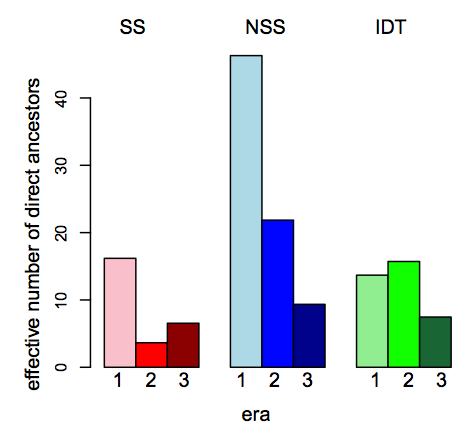
\includegraphics[width=0.45\linewidth]{joost_diversity.png}
\caption{Changes in genetic diversity (represented as the effective number of ancestors) of the three primary maize heterotic groups (SS: stiff-stalk; NSS: non-stiff-stalk; IDT: iodent). Inbreds are divided into eras representing different time periods: 1:1930-1950; 2:1950-1980; 3:1985-1992. Figure from \citet{van2012historical}.} 
\label{fig:diversity}
\end{SCfigure}

While open-pollinated varieties and exotic inbred lines represent a viable source of new diversity, these have been only sparingly used in the private sector due to their poor agronomic performance, photoperiod sensitivity, and the necessary generations of back-crossing to adapted lines required to incorporate useful alleles into high-performing temperate germplasm \citep{goodman1999broadening}.
In contrast, older U.S. inbred lines, though lower-yielding than their contemporaries, harbor novel genetic diversity of potential use for breeding \citep[e.g.][]{chen2012characterization,wisser2011multivariate}, but are already adapted to the U.S. cornbelt.  
Breeders have clearly been successful in advancing high-yielding germplasm and discarding ill-adapted material.
This does not mean, however, that all discarded material has little genetic merit --- beneficial alleles can be lost to genetic drift, particularly considering the polygenicity of agronomic traits and also because breeders are unable to select for all traits simultaneously. Our own population genetic analysis supports this notion; a number of underutilized older inbreds are enriched with favorable alleles (Figure \ref{fig:wf9}). 

\begin{SCfigure}
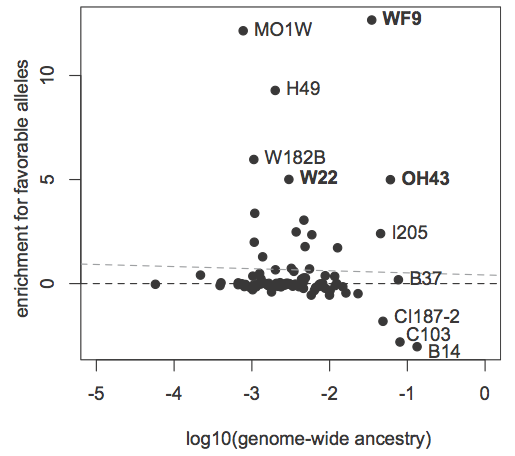
\includegraphics[width=0.55\linewidth]{joost_wf9.png}
\caption{Enrichment (log probability ratio with respect to control loci) of favorable alleles in older (era 1) inbreds as a function of average ancestral contribution to modern (era 3) lines. The gray dotted line is a  regression with slope $-0.1$). Inbred names are shown for lines with ratios higher than 4 or ancestry proportion above 0.03. Labels in boldface mark breeding lines of known historic popularity. Figure from \citet{van2012historical}.} 
\label{fig:wf9}
\end{SCfigure}

\subsection*{Lack of public resources limits use of diverse germplasm}

Breeders will not blindly incorporate older material into their populations, however.  
Perhaps the most important piece of information required to effectively utilize older germplasm is pedigree.
Pedigree data immediately gives a breeder information on crosses likely to produce higher yields due to heterosis, and often provides additional utility in identifying likely maturity (flowering time) and other agronomic characteristics. 
Combined with phenotype data, pedigrees can even be used to predict phenotype in the absence of genotype \citep{piepho2008blup} and pedigree-based methods for identifying useful diversity have already been patented by industry \citep{sebastian1995method}.

While private industry may in many cases have detailed records of their own breeding material, the vast majority of private germplasm is founded on $20^{th}$ century public breeding lines \citep{nelson2008molecular}.

Unfortunately, pedigree data for most U.S. maize inbreds is unavailable to most breeders. 
For example, of the over 45,000 worldwide inbreds in the USDA Germplasm Resources Information Network, only some 34,000 have some amount of ancestry determined, and much of this information is incomplete.
If we look at available germplasm only, that number shrinks to 2931 accessions with any available ancestry information.
While there are published compilations of germplasm, these are far from complete:  \citet{gerdes1993compilation}, for example, contains complete pedigree data for less than 20\% of the germplasm in the USDA database.
Moreover, what ancestry information that is available is not in electronic form nor easily accessible in any single resource.  
Instead, historical pedigree information exists primarily in the minutes of breeding committees, old breeding program books, and other hard-copy sources with limited distribution.  

\textbf{We propose to generate an open-source database of public maize pedigrees and use this resource to identify genotypic and phenotypic diversity of high utility in advancing maize breeding.}
Given the importance of maize to U.S. agriculture, this proposal clearly aligns with the USDA AFRI program priorities of ``Plant Breeding for Agricultural Production,'' particularly the ``development and application of tools to predict phenotype from genotype to accelerate breeding of finished varieties''.   
Our proposal will develop tools to accelerate breeding by allowing breeders to more quickly identify useful inbreds, and our application of population and quantitative genetic methods will identify specific genetic and phenotypic diversity of potential use for future breeding.  

\section*{Introduction}
\label{sec:introduction}

\subsection*{Maize breeding}
Maize has undergone dramatic phenotypic and genetic changes since its domestication and subsequent spread across the Americas \citep{daFonseca:2015ey,Doebley:2004ce}. More recently, beginning in the mid-20$^{th}$ century, the intensification of maize breeding efforts has lead to subtler but equally important changes including increasing yields and improved agronomic traits such as leaf angle and density tolerance \citep{duvick2005contribution}. 

Modern breeding programs (post-1960) take advantage of self-fertilization (or now double-haploid technology) to create homozygous inbred lines, which are maintained in separate breeding pools or heterotic groups.
The most important heterotic groups among U.S. public germplasm are the ``stiff stalk'', ``non-stiff stalk'', and ``iodent'' (Figure \ref{fig:diversity}).
Inbred lines from separate breeding pools are then crossed to make hybrid progeny.  
These hybrids often display heterosis, meaning that yield and associated traits of the hybrid are superior to  either inbred parent \citep{Springer:2007bj}.  
Inbreds capable of producing high-yielding, heterotic offspring are said to have good ``combining ability'', and are recycled in their respective breeding pools.
Inbreds that form less desirable combinations are usually discarded from the breeding pool. 
Useful inbreds within a group are crossed with each other, and their segregating progeny evaluated and self-fertilized to create new inbreds. 
Maintaining this system for propagation of inbred lines and hybridizing inbreds for evaluating production traits has worked well for many decades, but there is growing reason for concern that this method may need a genetic boost. 

\subsection*{Decelerating yield gains and decreasing diversity} 

Maize yields have steadily increased since the advent of hybrid breeding in the 1930's.
But linear increases necessarily mean a decrease in relative gain, and projections suggest that current trends are unlikely to meet future yield goals \citep{grassini2013distinguishing}. 
Of even greater concern is the possibility that the rate of gain may actually be decreasing (Figure \ref{fig:piecewise}).
While some of these yield trends are undoubtedly related to changing management practices, much of the change is indeed due to breeding \citep{Duvick:2001fy}, and current rates of yield gain are lower than historical trends even after correcting for nitrogen fertilizer inputs (data not shown). 

\begin{figure}
\centering
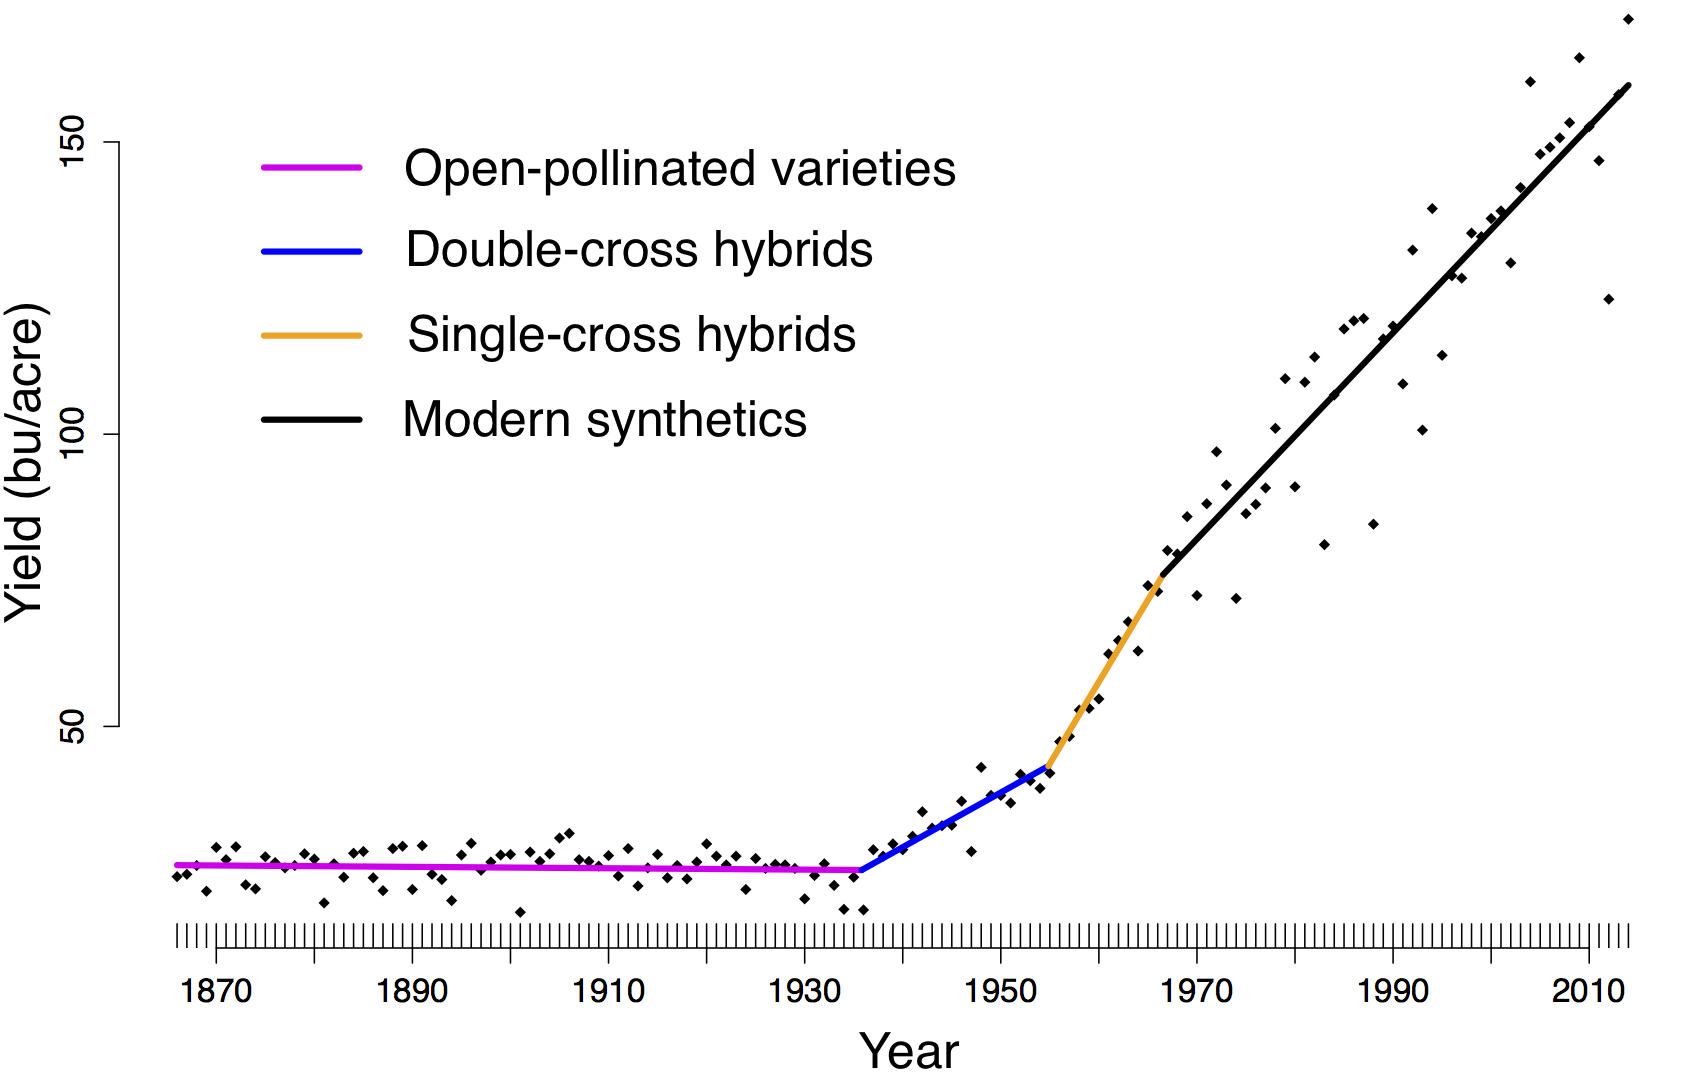
\includegraphics[width=0.7\linewidth]{yield.png}
\caption{Piecewise regressions of time against total yield through the four eras of modern maize breeding. Colors represent distinct eras of maize breeding that roughly correspond to the eras  referred to in Figure \ref{fig:diversity}.} 
\label{fig:piecewise}
\end{figure}

As selection progresses within a breeding program, inbred lines with poor performance are generally discarded, leading to a decreased effective population size ($N_e$) of the breeding pools.
Response to selection is proportional to the additive genetic variance $V_A$ (equation \ref{eq:lush}), and $V_A$, in turn, depends on $N_e$ as well as the mutational variance per generation ${\sigma}_m^2$ \citep{whitlock1999neutral}:

\begin{align}
E[V_a] = 4N_e {\sigma}_m^2
\label{eq:whitlock}
\end{align}

A reduction in $N_e$ thus inherently leads to a reduced response to selection, leading to diminishing returns on yield unless new diversity is brought back into breeding pools.
Evidence from the Iowa Reciprocal Recurrent Selection breeding program suggests these concerns are valid (Figure \ref{fig:trends}), as yield gains plateau over time \citep{rouse2003selection} concomitant with continued declines in genetic diversity \citep{Gerke:2013tw}.
Decreasing $N_e$ (Figure \ref{fig:diversity}) in U.S. cornbelt germplasm risks our ability to maintain or increase rates of genetic gain in yield.

\begin{SCfigure}
    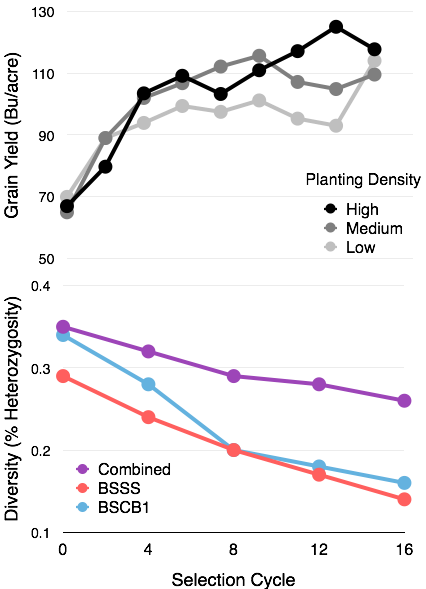
\includegraphics[width=0.45\textwidth]{BSSS.png}
  \caption{Yield and genetic diversity in the Iowa Recriprocal Recurrent Selection Program across 16 cycles of selection. (Top) Grain yield at three planting densities; data are from \citet{rouse2003selection}. (Bottom) Genetic diversity of the BSSS and BSCB1 breeding pools separately and combined; data are from \citet{Gerke:2013tw}.}
\label{fig:trends}
\end{SCfigure}

\subsubsection*{Useful diversity in old lines}
As any breeder will attest, old lines have fallen out of use precisely because they showed inferior agronomic performance under a particular selective regime (usually combining ability).
There are a number of reasons, however, why older lines may retain useful genetic diversity.
Lines are often discarded or selected against because of poor performance for a particular trait, but this does not preclude that line's utility in breeding for other traits.
Because of this, beneficial alleles for many traits of interest may remain in older germplasm, not having been advanced during breeding (Figure \ref{fig:div}).
For example, thanks to its combining ability, the U.S. inbred B73 quickly spread in popularity and now makes up a considerable portion of modern breeding material \citep{van2012historical}. 
Yet when evaluated for drought and heat stress, B73 significantly underperformed compared to less well-utilized lines such as B76 \citep{chen2012characterization}.
Analysis of a suite of diseases also finds that many less well-utilized public inbreds show greater resistance than popular lines \citep{wisser2011multivariate}. 

Most breeding programs consist of relatively small population sizes, and in these cases genetic drift can substantially impact the fate of even beneficial alleles \citep[e.g.][]{Gerke:2013tw}.
The contribution of older lines to modern germplasm thus does not necessarily reflect their genetic potential: our population genetic analysis of maize ancestry, for example, found lines with more beneficial (as defined by a steady increase in allele frequency over time) alleles than expected given their contribution to modern germplasm (Figure \ref{fig:wf9}).

\subsection*{A novel pedigree-based approach to incorporate new diversity}

Incorporating novel diversity into contemporary modern maize lines is clearly an important goal necessary to maintain or accelerate breeding and rates of yield gain.
While there are other public efforts that aim to achieve this goal, like the GEM  (Germplasm Enhancement of Maize) program \citep{pollak2003history}, these  focus on incorporating exotic germplasm (e.g. CIMMYT lines, tropical hybrids, etc.) into U.S. materials by backcrossing to well-adapted U.S. cornbelt backgrounds.
While this approach is successful at bringing in new diversity, it requires time-consuming back-crossing before it can generate lines that are of sufficient quality to incorporate into a breeding program.

\textbf{We propose a different approach, using pedigree data to identify underutilized cornbelt germplasm.}  
While this approach shares with projects like GEM the disadvantage that diverse material is often  agronomically inferior, it has a number of advantages.  
First, in contrast to exotic germplasm, older U.S. germplasm is already reasonably well-adapted to the daylength and climate of the U.S., meaning it can be immediately incorporated into breeding programs without first requiring extensive back-crossing.
Second, with sufficient information (see below), breeders may be able to learn a substantial amount about the potential utility of a line by predicting phenotype directly or understanding its relationship to known material. 
Finally, considerable information is available about many old breeding lines even without prediction (Figure \ref{fig:words})

\begin{figure}[t]
        \begin{subfigure}[b]{0.5\textwidth}
                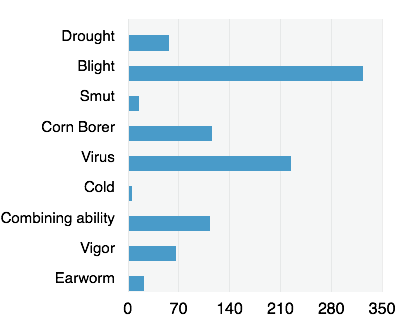
\includegraphics[width=\textwidth]{disease.png}
                \caption{}
                \label{fig:words}
        \end{subfigure}%
        ~ %add desired spacing between images, e. g. ~, \quad, \qquad, \hfill etc.
          %(or a blank line to force the subfigure onto a new line)
        \begin{subfigure}[b]{0.5\textwidth}
                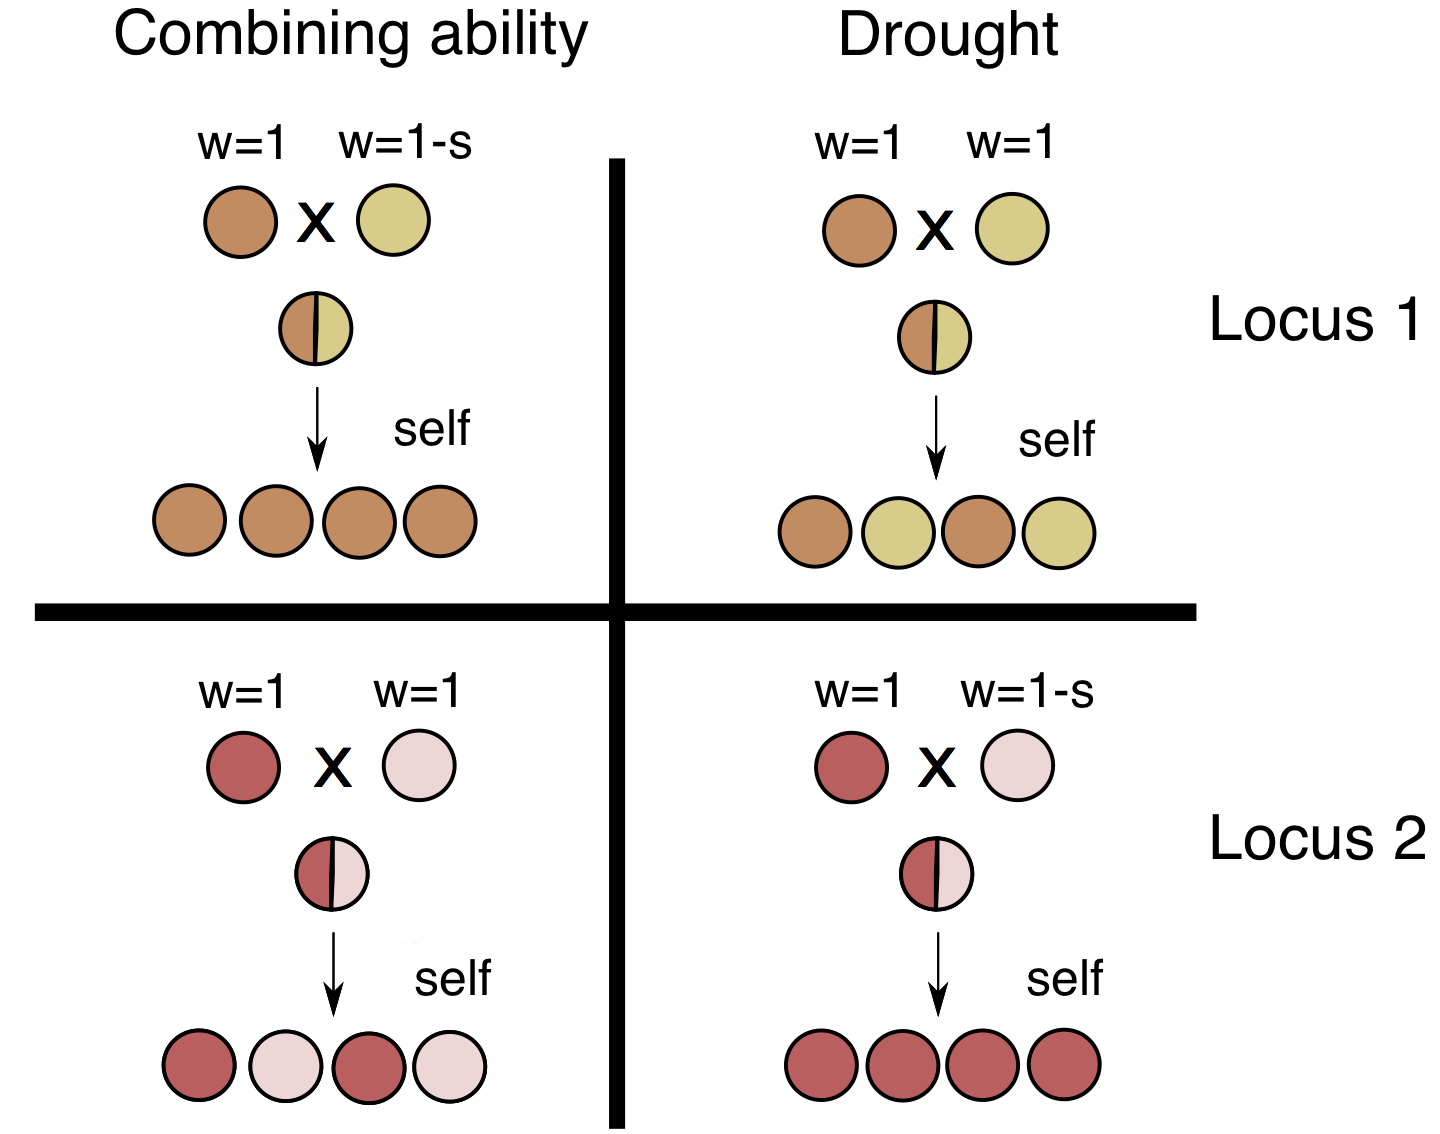
\includegraphics[width=\textwidth]{divergent.png}
                \caption{}
                \label{fig:div}
        \end{subfigure}
\caption{a) Counts of a small set of germplasm descriptors from the USDA database for which we currently have genomic and ancestral data. b) Expected segregation of alleles at loci for two traits in different breeding programs.  Selective regime for combining ability across two example breeding programs and loci. Fitness (w) of each allele indicated, with selection coefficient (1-\textit{s}) for the allele being selected against in a given regime. Locus 2, though beneficial under drought conditions, risks loss due to drift in breeding programs focusing only on combining ability.}
\end{figure}
 
\subsubsection*{Advantage of pedigree approaches}
\textcolor{red}{$XXXX--->$}
Most release sheets and information in NPGS on modern inbreds contain not only parentage information, but a wealth of important phenotypic information and the selective regime used in propagating a given line (e.g. Figure \ref{fig:words}). 

Using expectations of relatedness coefficients between known close relatives (inbred parents-inbred progeny) we can compare to observations of genomic sharing, where significant deviations from expected relatedness coefficients would tend to indicate selection. 
Across the entire pedigree, we expect that certain alleles will go to fixation due to breeder's selection as they are beneficial for ``combining ability''. 
But, within smaller breeding programs (and pedigrees) under a specific selective regime we will observe only 

CITE ZAMIR somewhere: zamir2013have

\begin{itemize}
\item observed vs. expected allow us to look allele specific ``hard'' breeder sweeps across the pedigree for combining ability
\item but phenotypic information of each program contained in release sheets may also allow us to look at selective regimes within programs (while selection is relaxed in others).
\item If alleles exist in other programs along with the specific diversity of that program, we can target those.
\end{itemize}
\textcolor{red}{$<---XXXX$}

\subsubsection*{The missing data challenge}

Unfortunately, much of the pedigree information on older founder inbred maize lines sits in old volumes of Crop Science or the Agronomy Journal, experimental station technical bulletins, regional corn breeding meeting records, release sheets, or breeding books --- unaviable and vulnerable to loss.  
The National Plant Germplasm Service (NPGS) database records ancestry information, but at least 25\% of the accessions in the database have zero ancestry data, and another \textcolor{red}{XXX} have incomplete data. 
While private companies likely have their own pedigree databases, these data are private, patented, and not available to the public. 
\textbf{We will gather pedigree data from public sources (minutes of breeding committees, breeding program books, and other hard-copy-only sources) in order to preserve this historical information and combine it with genotyping data to accelerate future public and private (see letter of support from Dupont Pioneer) maize breeding programs.}

\subsection*{Preliminary work}
To date, we (senior personnel Drs. Oscar Smith and Kate Crosby) have gathered parentage info for over 3193 lines from a variety of sources, including \cite{gerdes1993compilation}, the NPGS, patent variety protection records, inbred release publications, and communication with breeders.
We have standardized names across these datasets and stored these data in a SQL database, which can be queried by common name (e.g. ``B73'') as well as unique NPGS identifiers (``PI 550473'' for B73).
We have combined these data with genome-wide genotyping-by-sequencing (GBS) data \citep{romay2013comprehensive}, and built a large pedigree of $\approx$700 lines (Figure \ref{fig:combo}a) with complete parentage and genotype information. GBS data allows us to validate recorded pedigrees, identifying parental combinations that are impossible given the genotyping data (Figure \ref{fig:combo}b).

\begin{figure}
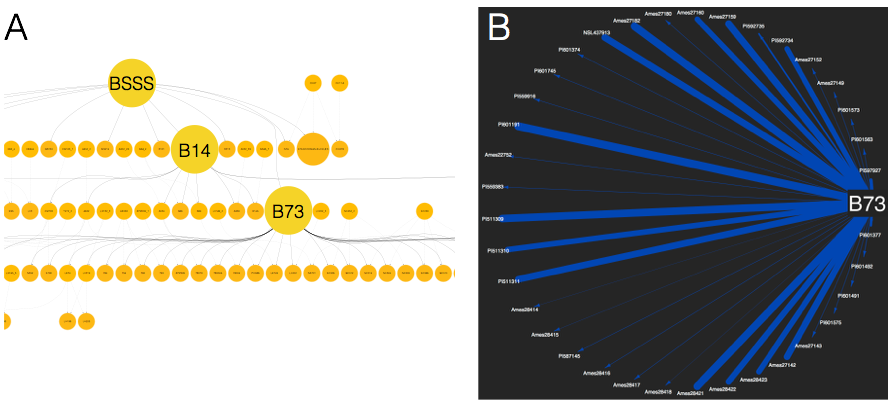
\includegraphics[width=1\linewidth]{crosby_combo}
\caption{A) A small portion of our current pedigree, showing partial data for inbred  B73. B) Pedigree of putative first-generation descendants of inbred B73. Blue arrows are weighted by the relatedness estimated from identy-by-state using GBS, clearly showing multiple errors in the putative pedigree.}
\label{fig:combo}
\end{figure}

\section*{Approach}
\label{sec:approach}
Our proposed research has three major aims in identifying and utilizing diversity to accelerate maize breeding.

\begin{itemize}
\item Aim 1: Digitize and curate pedigree and genotype information into a publicly available database. 
\item Aim 2: Identify useful diversity using a combination of pedigree and population genetic approaches.
\item Aim 3: Field test individuals lines that feature heavily in the historical pedigree.
\end{itemize}

\subsection*{Aim 1: Public pedigree curation}
Our first aim is stop the potential loss of hard copy pedigree data by gathering it from land grant institutions that previously hosted breeding research programs of maize inbred lines. 
Land grant schools of primary importance were identified by Co-PI Dr. William Tracy and  Dr. Smith (senior personnel), who have between them have more than 70 years of breeding experience in maize. 
Dr. Tracy was senior author on the leading pedigree book of maize lines \cite{gerdes1993compilation} and Dr. Smith spent 7 years working as maize breeder for the USDA (including working on the Iowa RRS population), follow by more than 20 years as a maize geneticist for Dupont Pioneer. The land grant schools they have identified include: the University of Wisconsin, Virginia Tech, the University of Georgia, the University of Florida, Pennsylvania State University, the University of Nebraska, North Carolina State University, and the USDA station at the University of Missouri. 

Co-PI Tracy and Co-PI Holland's student will largely be responsible for visiting these schools in the first year to obtain and digitally scan this information with portable digital scanners. 
Co-PI Wisser's student will be responsible for visiting two schools starting in the second year of the grant.
Co-PI  Tracy will obtain information from the University of Wisconsin (host institution), the University of Florida, and the University of Nebraska. 
Co-PI Holland's student (in the first year) will be responsible for North Carolina State University (host institution), the University of Georgia.
Dr. Sherry Flint-Garcia (senior personnel) has agreed to obtain and pass along records from the USDA station at the University of Missouri. 
Co-PI Wisser's student (to start in year two of the grant) will be responsible for the University of Pennsylvania and Virginia Tech.
Drs. Tracy and Smith have extensive contacts with faculty past and present at these schools, so obtaining the information and scanning it at each school traveled to should take no more than a few days. 

Optical character recognition software will be used where possible to automate extraction of information from scans, but we imagine a fair amount of hand-curation will be required.
Dr. Kate Crosby (senior personnel), Dr. Taner Sen (support letter from maize GDB enclosed), senior personnel Dr. Oscar Smith, and Co-PI Dr. Bill Tracy will consult on an agreed upon standard format for recording data from scans.
Standardized formatting will enable consistent mapping of current and future genomic data formats to pedigree information. Both the raw scans of pedigree records and our data sheets which will be made available publicly with permanent doi via services such as Github (\url{www.github.com}) or Figshare (\url{www.figshare.com}).
We will translate current and new phenotypic data into standardized maize ontologies such as those supported by the Generation Challenge Program \citep[\url{http://www.cropontology.org/ontology/CO_322/Maize}, ][]{shrestha2012bridging}

We anticipate that we will identify some lines that feature heavily in the historical pedigree but that do not have any genotypic data available for them. 
To facilitate downstream applications (see Aims 2 and 3), we will use genotype-by-sequencing (GBS) \citep{Elshire:2011ha} to obtain genome-wide genotype data.
Germplasm will be requested from the relevant sources, and germination and DNA extraction will be performed at UC Davis.  
Genotyping will be outsourced to the Genomic Diversity Facility at Cornell University (\small{\url{www.biotech.cornell.edu/brc/genomic-diversity-facility}}), and sequence data processed following standard pipelines \citep{Glaubitz:2014eu}.
We anticipate that no more than a few hundred inbred lines (2-4 96-well plates) would need to be 

Dr. Crosby will be responsible for database generation and curation.
The initial database will continue to be in SQL format, with entries for release dates, historical phenotype information, breeder notes, germplasm availability (or nearest neighbor germplasm availability), and GBS genotype.  
While other genotyping has been performed on a number of lines, GBS is the \emph{de facto} standard \citep{romay2013comprehensive} and merging data across platforms is beyond the scope of the work proposed here. 
GBS data will be stored in hdf5 format and made available via iPlant (\url{www.http://iplantcollaborative.org}).
We will develop software to extract genotype data from specific genomic regions in subsets of lines and estimate allele sharing via identity by state (IBS) between sets of lines in specified genomic regions.
Finally, we will implement simple phenotypic prediction (see Aim 2) functionality allowing users to estimate phenotypic values based on a set of loci from genome-wide association studies.

Starting in year two of the grant, the pedigree database will be made available publicly via MaizeGDB (\url{www.maizegdb.org}), the USDA-funded central resources for maize genomics (see letter of support from Dr. Taner Sen).
We will update the database as new information arises, and provide functionality such that users can submit database updates (in the appropriate format) to MaizeGDB to ensure continued utility and availability of this resource.

\subsubsection*{Expected outcomes (Aim 1)}
Our main deliverable from Aim 1 is an \textbf{open public pedigree database to be hosted on MaizeGDB (http://www.maizegdb.org/) for the long term future.} 
Users will be able to contribute and revise incomplete information, with the goal of establishing a nearly complete public pedigree of maize inbred lines.   
For instance, a breeder could query the database for lines with descriptors suggesting drought and blight resistance, identify the genotype of such lines at loci thought to be associated with the trait of interest from GWAS or other studies, and use the database to predict phenotype for related material with no descriptive data.

Ensuring data, code, and script are open-access or open-source (freely available to the public) is important for critique, debate, and dialogue in science. 
Drs. Ross-Ibarra and Crosby have a long track record of ensuring openness in science, data, and code. Throughout this project, both Dr. Ross-Ibarra and Dr. Crosby will endeavour to ensure that code and data are available via permanent, publicly accessible repositories such as github, figshare, maizeGDB, and iPlant.

\subsubsection*{Potential pitfalls \& limitations (Aim 1)}
\textcolor{red}{While we are very optimistic about the prospect of obtaining accurate pedigree information from these various institutions the nature of corn-breeding and record keeping of corn-breeding can be nebulous. 
Ideally, we would be able to accurately count the number of meioses in the total pedigree, in each breeding program, down to each line; thus, retracing the complete ancestry of a given contemporary inbred. }


%JRI: DITCH THIS
%However, in many cases, it may not have been noted at which point in a breeding program a line was bulked at, nor on occasion which lines were used in recycling an inbred when seed was exhausted. 

%For instance, a record from NPGS may indicate that a line was bulked and stored after being selfed to generation 6, or it may have been bulked and stored following selfing at generation 4. As a ballpark figure, a ``selfed generation 6 inbred'' means that germplasm from that line is 99\% homozygous at all locus pairs. 
%Meaning that if this inbred is selfed further, not much changes with respect to levels of homozygosity nor heterozygosity (as recombination via selfing is ineffective beyond this point).  
%Thus, so long as an inbred is at or beyond cycle 6, it will be kept, but inbreds before this period shall be discarded.

%To ensure that historical records of inbred lines are isolated following the sixth generation of selfing and beyond we will investigate the level of heterozygosity in each of these lines with GBS data relative to the total amount of missing data in an individual line. 
%Within reasonable confidence limits most lines should show a very small portion of heterozygous loci even with GBS markers (known to have a high rate of error in the under-calling heterozygous). 

Historical pedigree records and other information on old lines may be available, but the germplasm from these old lines may no longer be available. 
Approximately 12.9\% of germplasm from NPGS for which we have parentage information is no longer available, and we expect similar or higher levels from less accessible sources. 
We note, however, that such lines remain useful in connecting available lines together in the pedigree, and pedigree alone can be used to predict phenotype. 
If we identify historically important germplasm that is no longer available, we will identify and genotype the nearest relatives for which seed are available. 

\subsection*{Aim 2: Identify useful diversity}

\subsubsection*{Mendelian segregation on a pedigree}
As different lines have been under different historical selective regimes or breeding programs, these phenotypes likely have an underlying genetic basis. Following the digitization of historical information, the Dr. Holland's student and the post-doc (Kate Crosby) will construct many small pedigrees of the different selection regimes and use the technique of \textbf{``allele-dropping''} to further identify breeder's selection and useful diversity. 

``Allele-dropping'' is a patented method \citep{sebastian1995method}, used in industry and works by identifying distorted segregation at all heterozygous loci within a single pedigree/breeding programs and across many pedigrees/breeding programs (Figure \ref{fig:alleledrop}). 
As a simple Mendelian approach this technique identifies traces of selection by directly accounting for ancestry, and without the worry of having to account for shared population structure \cite{sebastian1995method} (as can often be a problem or limitation in modern population genomics approaches). 

If we observe the uni-directional shift of a given allele across many of these small pedigrees at a set of loci (or even within just one pedigree in a specific breeding program), this would tend to indicate selection. 
We would tend to predict that a consistent subset of alleles that are associated with combining ability would tend to increase in frequency across the pedigree.
As an example, using Mendelian rules and starting with a mostly homozygous line (with some residual heterozygosity), we can examine single heterozygous locus (i.e. $Aa$). 
Because we know what our expectations ($E$) for number ($N$) of $AA$ (or $aa$) homozygous inbred progeny at generation 6 (under no selection) should be (given by $E = 1/2 N$), we can compare to the actual observed number of progeny. 
If our observations deviate from this expectation, we would tend to conclude breeder's selection for these alleles (especially if observed across a good portion of the entire pedigree). 

\begin{figure}
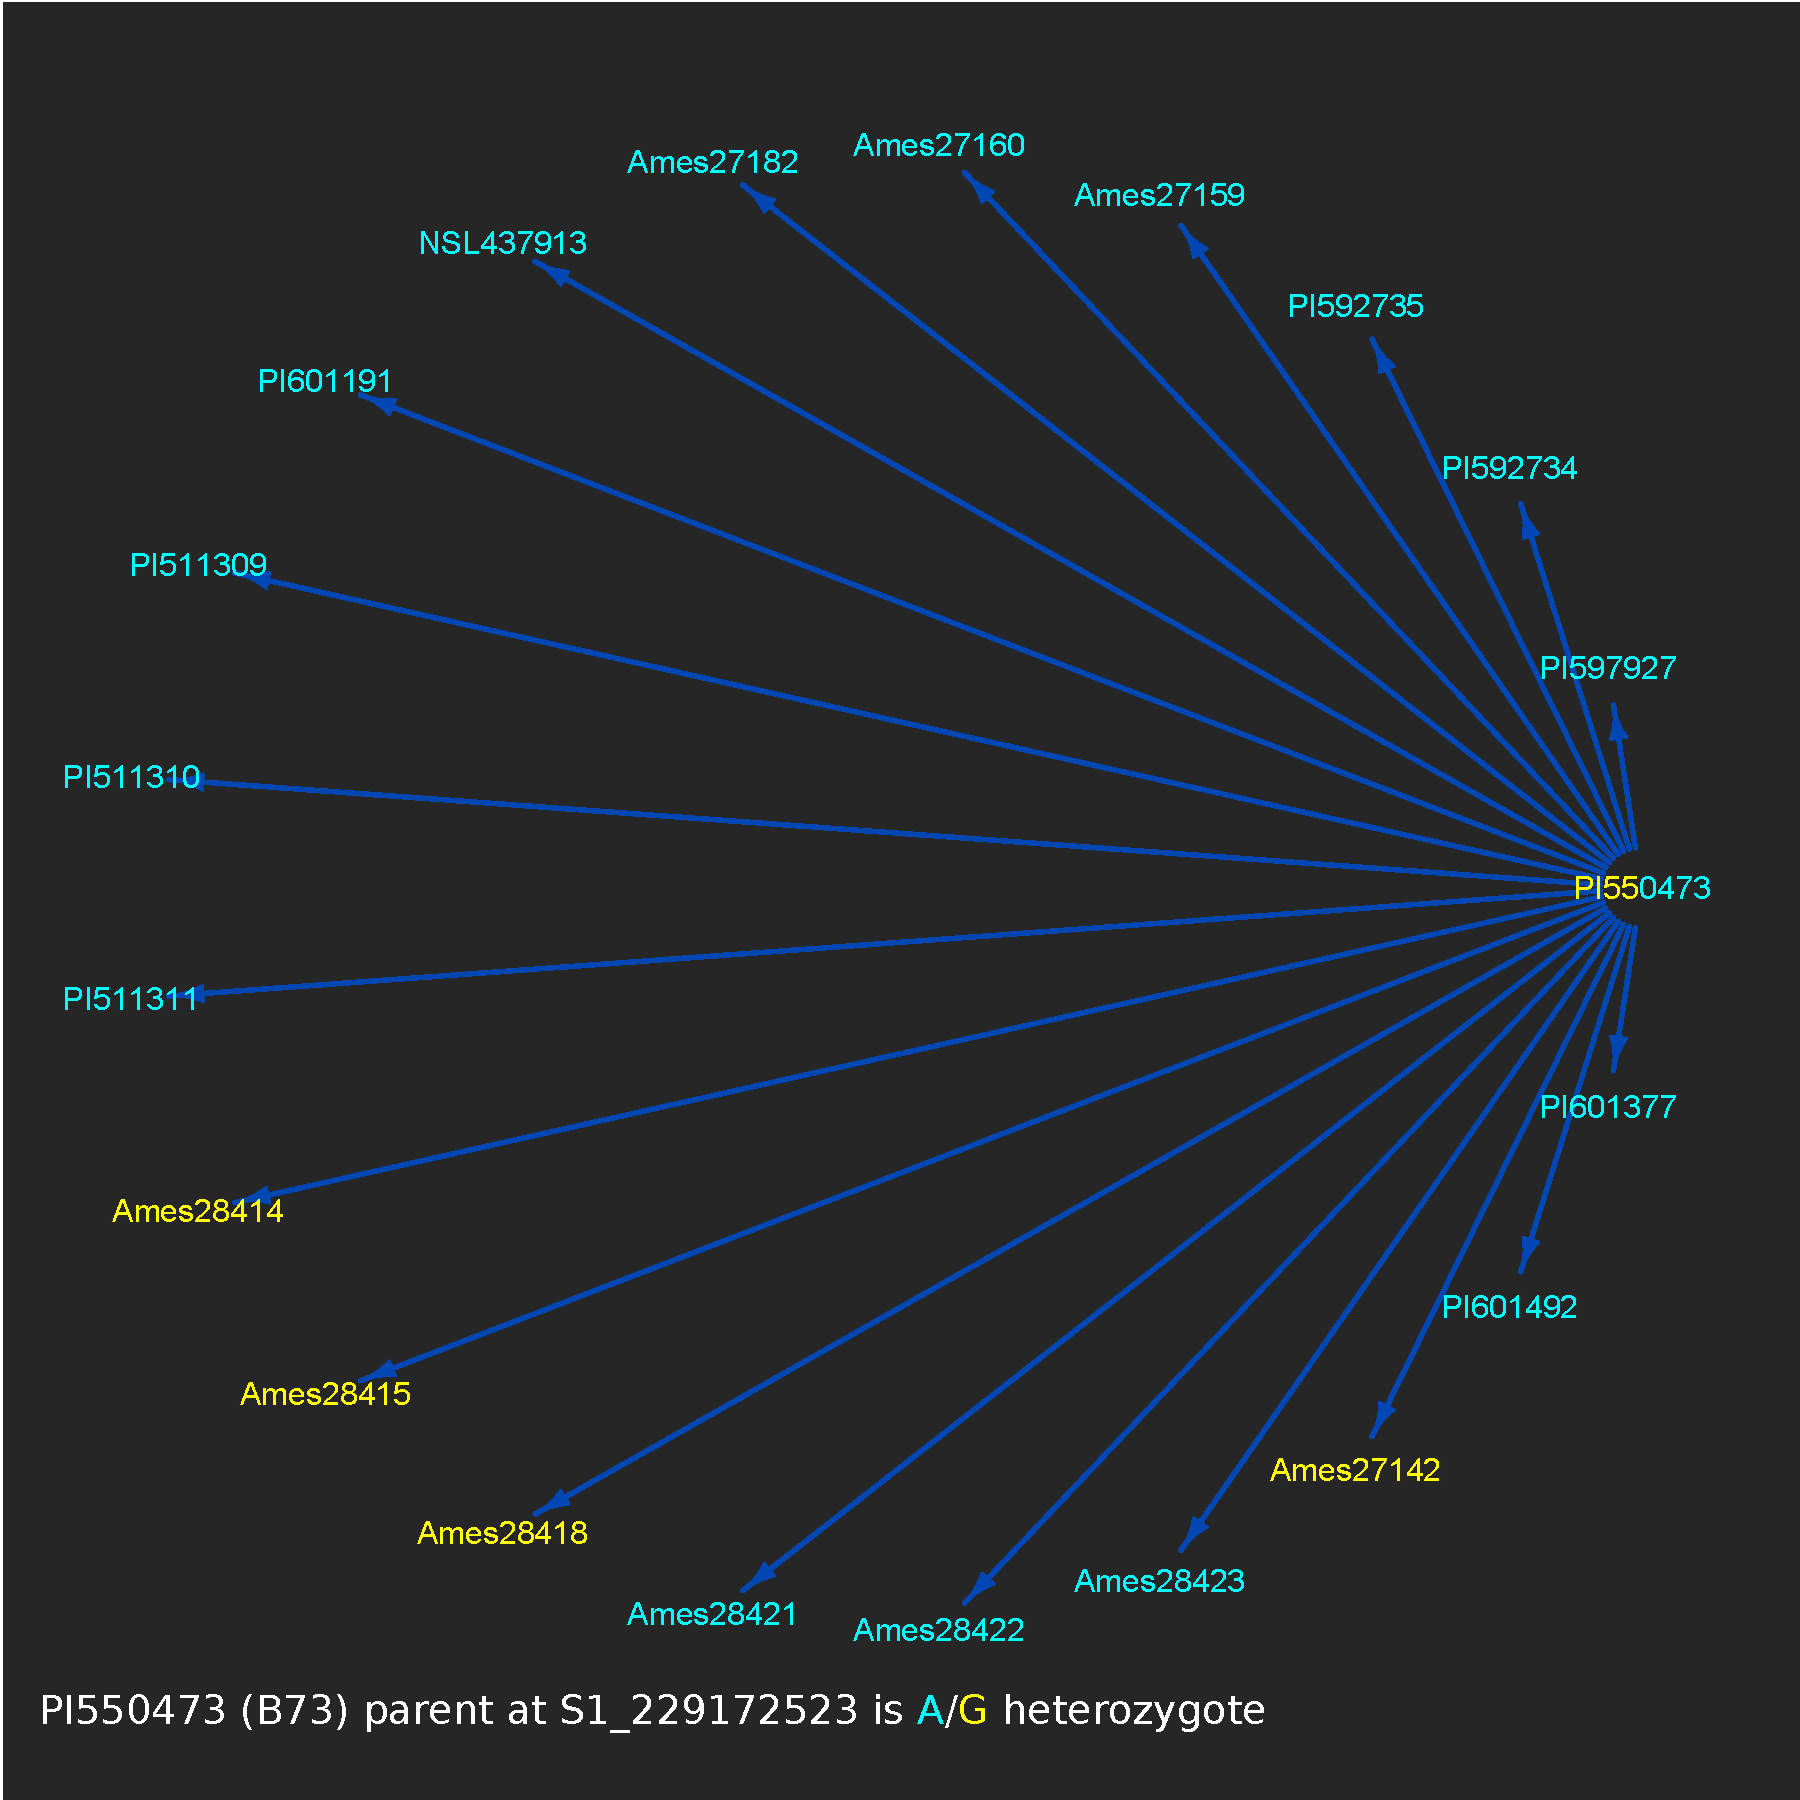
\includegraphics[width=0.5\linewidth]{Pruned.pdf}
\caption{B73 (also known as PI550473 by NPGS and a number of its inbred progeny) is heterozygous at 379 loci out of over 954,000 loci with GBS markers). The blue labels represent which inbred progeny obtained the A allele, whereas the yellow labels indicate the progeny that have obtained the G allele at a particular locus. \textbf{NB: the other parent of these lines is not indicated for simplicity}.}
\label{fig:alleledrop}
\end{figure}

Our current preliminary data set of 1696 accessions contains a fair amount of information on different selection regimes (Figure \ref{fig:words}). 
By applying allele-dropping to a number of these smaller breeding programs, and tracking unidirectional shifts, we (Dr. Holland's student and Dr. Crosby) will attempt isolate strong signals of breeders selection for a given selective agent (within a past breeding program). 
We may then look for these alleles across all other breeding programs where selection was presumably relaxed (Figure \ref{fig:div}), and if we can isolate these alleles, then they may be introgressed back in as useful diversity to other breeding programs.

\subsubsection*{Potential pitfalls \& limitations (allele-dropping)}
Genotypes when combined with a pedigree can be used to predict phenotypes \citep{de2009predicting,crossa2010prediction,Decker:2012kd}.
By using allele dropping we target individual loci within and across breeding programs, attributing high frequency SNPs with their given breeding program. 
However, there are two potential limitations with the allele-dropping approach. First, there may be a lack of statistical power in detecting selection on individual alleles, because there may be too few progeny of each line under a given selection regime. 
But, allele dropping may not have the statistical power to detect a more diffuse polygenic signal of adaptation spread across many alleles in a genome (similar the drawbacks of using traditional QTL mapping and $F_{ST}$ scans) \cite{Rockman:2011ej, Berg:2014bs}. 
However, this limitation of power is not an issue for the complementary population genetic approach we plan on using: the $Q_{x}$ method described in \cite{Berg:2014bs} (see next section). 

\subsubsection*{Predictive phenotyping ($Q_{x}$)}954
\jri{here we show that if individual lines predictive phenotype is better than expected given pedigree/genomic background, then it's likely a good choice for breeding! }

Here we propose the first study to look for correlated allele shifts (thought to be associated with production traits) in lines from different time periods (environments) using a statistic in a recently described population genomics approach \cite{Berg:2014bs}: $Q_{x}$. 
Briefly, the approach $Q_{x}$ takes SNP hits and their effect sizes from a GWAS analysis for observed phenotypic traits of interest in one environment, then projects the expected phenotypic (breeding) value based on the genotype of individuals in another environment (where the phenotype has not been observed). 
In the case of maize, we have contemporary lines from various mapping populations, their genotypes, and their phenotypes, e.g. the Nested Association Mapping population (NAM) \textcolor{red}{CITE NAM original ref}.   
First, significant hits from a genome wide association study (GWAS)  can be summarized as the allelic effects $\alpha^{2}$ (or breeding values) that breeders can take advantage to get an estimate of $V_{A}$ for any trait of interest. $V_{A}$ can be estimated for one locus or summarized across all loci $L$ in the genome (equation 3 below):

  \begin{align}
    V_A = 2pq\alpha^2
 % \end{equation}\break
 % \begin{equation}
     = \overset{L}{\underset{l=1}{\sum}}\alpha^2_l2p_l(1-p_l)
  \end{align}

If alleles are at high frequency in certain breeding programs and can also associated with a beneficial phenotype (e.g. blight resistance), they are potentially beneficial alleles that could be resurrected and introgressed back into a modern breeding program. 
By then searching the entire pedigree for these alleles and isolating those lines that have these SNPs, they may be targeted by breeders and public research programs.
Further, the greater the $V_A$ of a trait (the greater the allelic diversity of that trait, i.e. $N_{e}$), and thus, the greater $R$ (response to selection) to any new selective program a breeder chooses to apply.


\subsubsection*{Expected outcomes (Aim 2)}

The idea of applying these two complementary approaches is \textbf{the isolation of a consistent subset of SNPs within and across breeding programs}. 
These SNPs can then be tagged in the database as being important for yield-related traits under different selective pressures.
In obtaining this set of SNPs, each of the masters students will be trained in separate but complementary population and quantitative genetics approaches, and provide them with a skill-set for applied industry or public research. 


\subsection*{Aim 3: Field testing individual lines}
A mass grow out and genotyping of all inbred lines in the total pedigree would be ideal, but realistically, we do not have the resources (either in terms of time, space, or available germplasm) to do this.
However, we can target specific lines that have many progeny (thus, many alleles) or very few progeny (few alleles in the pedigree). These lines will have been identified with the allele-dropping method by Dr. Holland's student and Dr. Crosby. 
In the latter part of the second year, Dr. Wisser and his student will grow out several hundred of these lines, obtain tissue for GBS (for those with no genotypic information), and potentially also verify the phenotypic information provided on the release sheet (if the information is available). 

In order to empirically (\kc{right word?}) test and ground-truth the idea that inbred lines from the past express the predicted phenotypes from the $Q_{x}$ approach Dr. Wisser and his student will grow out a subset of lines in the third year at the University of Delaware, and phenotype these.
The subset of lines here will be based on those lines that show overdispersion for production and production associated traits from the $Q_{x}$ approach described above, and ``fit'' and ``unfit'' lines from the allele-dropping method. 
We have allocated resources to grow out 50 of the predicted ``fit'' and 50 ``unfit'' lines, with 2 rows of 10 each, and the middle 5 of each row will be phenotyped. 
We will include several contemporary ex patent-variety-protection (ex-PVP) lines to check the predictions given by $Q_{x}$.


\subsubsection*{Expected outcomes and potential pitfalls: Aim 3}
This final aim of the project fills in any incomplete genotype and phenotype information for important lines in the pedigree. If the ``best old'' lines show terrible agronomic performance, we will know the approach of integrating ``old'' diversity is an inefficient approach to adding diversity to the breeding pool for yield. 
We expect that it will demonstrably provide evidence of breeder's selection through time on different lines.
Perhaps, more importantly, it will allow us to evaluate the expected/predicted effects sizes (breeding values) of an identified SNP on the observed phenotype. 



\subsection*{Timeline}
\kc{A graphical timeline of our three-year proposal WILL BE presented below}. 

The first year will be spent traveling and gathering and digitizing pedigree records at land-grant institutions.
Dr. William Tracy and Dr. James Holland's masters student will be responsible for traveling to and scanning hard-copy records into digital format.  We estimate that this should take no longer than a few weeks at each institution with the first student or CO-PI. 
The scanned digital records must then be translated into a usable data format for further analysis with NGS or phenotype data. At worst, this will involve the student, CO-PI (Holland or Tracy) or the postdoc (Crosby), physically reading and translating each of the scanned papers, and this could take several months to the entire first year depending on volume of records. 
At the end of the first year/start of the second year, any inbred line that is disproportionately present or absent in the pedigree with available germplasm, but that has no to little genetic information on it will be genotyped using the GBS platform. 
Dr. Holland's student will begin to apply the technique of allele-dropping to various pedigrees and associating these
Dr. Randall Wisser's student will then start and visit the two land grant schools in the east (Virginia Tech and the University of Pennsylvania) to obtain the remaining record, and submit this phenotypic and pedigree information to the up-and-running database in the first 2-3 months. Following this, he/she will (over a period of 2-3 months) learn the population genomics approach presented in \citep{Berg:2014bs},


\newpage
\bibliography{kc.bib,jri.bib}
\end{document}